% !TEX root = thesis-ex.tex

\section{Quantum Chromo-Dynamics}

Quantum Chromo-Dynamics (QCD) is a relativistic non-abelian gauge theory, with symmetry group SU(3), which describes the strong interaction between quarks and gluons. Quarks are charged subatomic particles that are the fundamental constituents of matter and gluons are gauge bosons that are mediators of the strong interaction between quarks. In its form, QCD appears similar to QED~\cite{Seymour:2005hs}, however, since the gluons of the strong force carry color charge, solutions to the QCD Lagrangian become more complicated. The QCD Lagrangian~\cite{qcdbook} is 

\begin{equation}
\mathcal{L}=\bar{\psi}_{i}(i\gamma^{\mu}\partial_{\mu}-m_{i})\psi_{i}-g\bar{\psi}_{i}\gamma^{\mu}t_{ij}^{a}\mathcal{A}_{\mu}^{a}\psi_{j}-\frac{1}{4}F^{\mu\nu}_{a}F_{\mu\nu}^{a},
\label{eq:lagrangian}
\end{equation}

where $\psi$ is the spin-1/2 quark field (quark), $m_{i}$ is the quark mass,  $\mathcal{A}_{\alpha}^{A}$ is the spin-1 gluon field (gluon), $t_{ij}^{a}$ is a generator from the fundamental representation of the $SU(3)$ group which describes the interactions between quark and gluon fields. The field strength tensor $F^{\mu\nu}_{a}$ is derived from $\mathcal{A}_{\alpha}^{A}$,

\begin{equation}
F_{\mu\nu}^{a}=\Big[ \partial_{\mu}\mathcal{A}_{\nu}^{a} - \partial_{\nu}\mathcal{A}_{\mu}^{a} - g f^{abc}\mathcal{A}_{\mu}^{b}\mathcal{A}_{\nu}^{c}\Big]
\label{eq:fieldtensor}
\end{equation}

where the indices $a$, $b$, and $c$ sum over the eight color degrees of freedom of the gluon field and $f^{abc}$ are the structure constants of the $SU(3)$ color group. The term $g=\sqrt{4 \pi \alphaS }$ is related to the strong force coupling constant \alphaS.

\begin{figure}
	\centerline{
		\includegraphics[width=0.6\textwidth]{figures/asq-2015.pdf} 
	}
	\caption{Strong force coupling constant \alphaqs, which decreases with increasing four-momentum transfer $Q=\sqrt{|q^{2}|}$.  Figure taken from Ref.~\cite{pdg:2018}.}
	\label{fig:strongforceconstant}
\end{figure}

In~\ref{eq:lagrangian}, the left-most term, $\bar{\psi}_{i}(i\gamma^{\mu}\partial_{\mu}-m_{i})\psi_{i}$, is the Dirac equation describing a free particle. To account for interactions with the field, additional terms are present. The middle term, $g\bar{\psi}_{i}\gamma^{\mu}t_{ij}^{a}\mathcal{A}_{\mu}^{a}\psi_{j}$, describes the coupling between quarks and gluons, and the last part of the Lagrangian, $\frac{1}{4}F^{\mu\nu}_{a}F_{\mu\nu}^{a}$, is the kinetic term from the gluon field. 

The third term, $f^{abc}\mathcal{A}_{\mu}^{b}\mathcal{A}_{\nu}^{c}$, in the field strength tensor $F^{\mu\nu}_{a}$, is the non-abelian term that distinguishes QCD from QED. This gives raise to three- and four-point gluon vertices, resulting in the three basic vertices of QCD, shown in Figure~\ref{fig:qcdvertices}. 

\begin{figure}
	\centerline{
		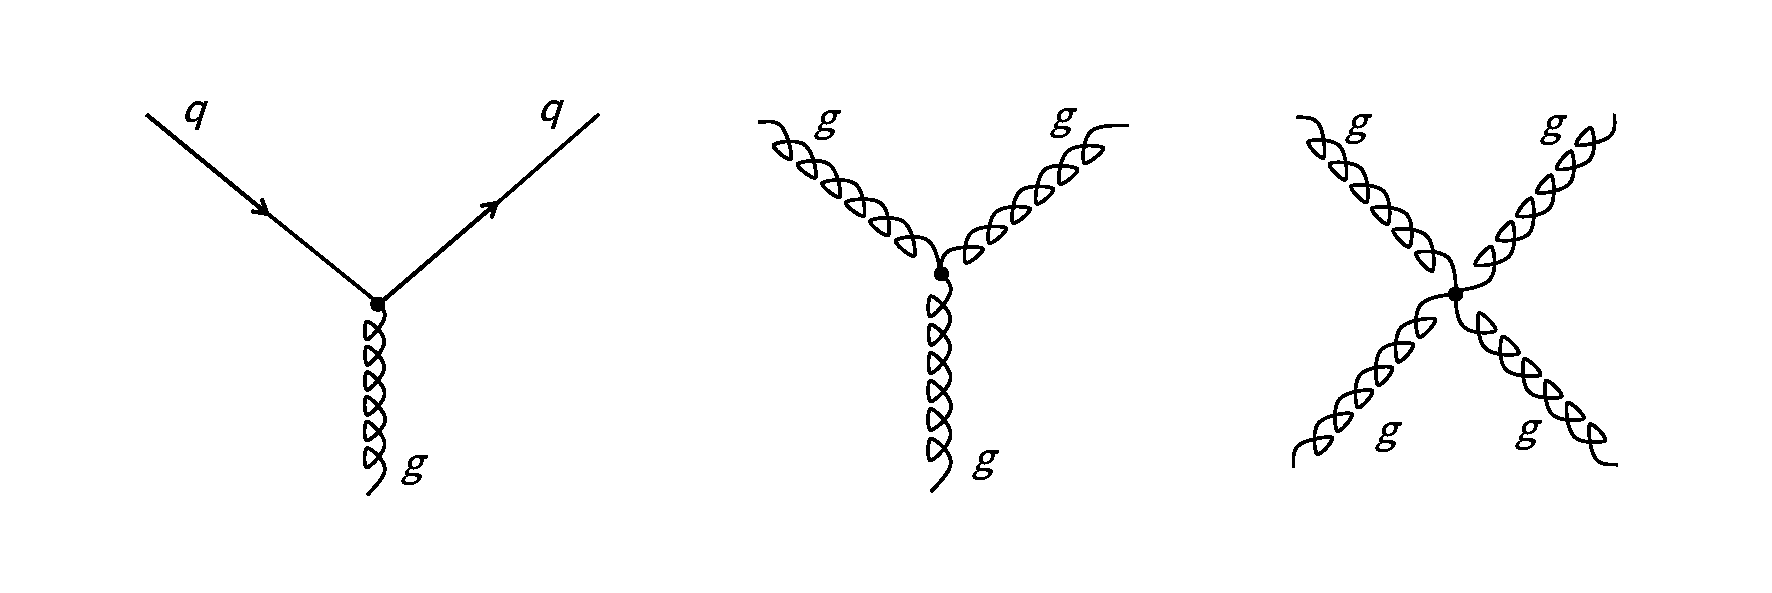
\includegraphics[width=0.9\textwidth]{figures/qcd_vertices.pdf} 
	}
	\caption{Three types of QCD vertices: the basic quark-gluon QCD vertex (left), three-gluon self interaction (center), and four-gluon self interaction (right). }
	\label{fig:qcdvertices}
\end{figure}

A consequence of gluon self interactions in QCD is the fundamental property of asymptotic freedom: the fact that the strong force coupling constant \alphaqs\ decreases with increasing energy scales, or by the uncertainty principle, smaller distances. The four-momentum transfer $Q=\sqrt{|q^{2}|}$, where $q$ is the four momentum of a virtual particle responsible for an interaction, determines the energy and distance scales ($d\sim 1/Q$) probed. Asymptotic freedom also explains the interpretation that quarks and gluons are point-like particles since the distances probed inside the proton can be arbitrarily small. The behavior of \alphaS\ at larger distances, or smaller energies shows a rapid increase in the coupling between quarks and gluons. A direct consequence of this is that particles which interact via the strong force are highly confined: they cannot exist freely at macroscopic distances. Only color singlet states - quark-antiquark pairs (mesons) and three quark states (baryons) exist stably~\cite{Seymour:2005hs}.  The behavior of \alphaS\ is shown from various measurements as a function of four-momentum transfer $Q$ in Fig.~\ref{fig:strongforceconstant}. 

There have been several techniques developed for performing QCD calculations. The two established methods are perturbative QCD (pQCD)~\cite{Brock:1993sz} and lattice QCD~\cite{creutz1985quarks}. Lattice QCD is used predominantly for calculations at lower energies where \qsquare\ is small and \alphaS\ is large. These calculations are performed below the characteristic QCD scale $\lambda_{QCD}\sim200$ MeV, where $\alphaS\sim 1$. Lattice QCD calculations have been successful in describing experimental data on the properties of nucleons, such as their mass mass~\cite{Borsanyi:2014jba}. Additionally, these computationally intensive calculations support experimental evidence of a new state of matter that exists at high temperatures and densities called the Quark Gluon Plasma (QGP)~\cite{Harris:1996zx,Adcox:2004mh,Adams:2005dq,Arsene:2004fa,Back:2004je}. If the \qsquare\ of a system is above $\lambda_{QCD}$, meaning \alphaS\ is sufficiently small, pQCD calculations can be used because an order-by-order expansion of the Lagrangian in powers of \alphaS\ is appropriate. In this high \qsquare\ regime, individual quarks or gluons in the nucleus can be resolved. Whereas, in the low \qsquare\ regime, where lattice QCD calculations are used, only individual nucleons and not their constituents can be observed. The measurement presented in this dissertation will rely on tools that were developed to work at energy scales where pQCD calculations can be used.

\begin{figure}[hb]
	\centerline{
		\includegraphics[width=0.65\textwidth]{figures/dis_2.pdf} 
	}
	\caption{ The DIS process that takes place in $e^{\pm}p$ collisions with an exchange via a virtual photon $\gamma^{*}$. Figure taken from Ref.~\cite{Iancu:2012xa}. }
	\label{fig:dis}
\end{figure}


\section{Deep Inelastic Scattering}

The proton, the fundamental building block of nuclear matter in nature, is a fermion with one positive unit of electric charge, a spin of $1/2 \hbar$. However, much more has been discovered about its fundamental properties and constituents in recent years. Almost half a decade ago the so called $naive\ parton\ model$~\cite{Bjorken:1969ja,Peskin:1995ev} of the proton was proposed: the proton was made out of non-interacting point-like constituents called partons, which were thought to be charged fermions, possibly bound together by some other neutral particles. This model was first supported by evidence from through lepton-nucleon Deep Inelastic Scattering (DIS) experiments from the SLAC-MIT collaboration~\cite{Whitlow:1990gk}. Commonly, this was done with an electron and a proton, with incoming four-momenta $e$ and $P$, respectively, and a virtual photon with four-momentum $q$ acting as the exchange particle. This process, $ep \rightarrow eX$, where $X$ are the remnants of the proton, is shown in Fig.~\ref{fig:dis}. From these quantities, we define two important variables in DIS, the first is the proton longitudinal momentum fraction carried by its constituent parton, $Bjorken$-\xb:

\begin{equation}
\xb = \frac{\qsquare}{2P\cdot q} = \frac{\qsquare}{2M\nu},
\label{eqn:xb}
\end{equation}

where $\nu$ is the energy of the virtual photon in the proton rest frame. The second variable is the lepton momentum fraction transferred to the proton:

\begin{equation}
y = \frac{P\cdot q}{P \cdot e} = \frac{\nu}{E},
\label{eqn:ydis}
\end{equation}

where $E$ is the energy of the lepton in the proton rest frame. The resolving power of the photon goes as $R^{2} \sim 1/\qsquare$, meaning that for the proton, with a proton radius of $R_{p}\sim8$ fm, if $\qsquare \equiv -q^{2} \ll 1\ \mathrm{(GeV/c)^2}$, the photon will interact elastically with the proton nucleus as a whole. If $\qsquare \equiv -q^{2} \gg 1\ \mathrm{(GeV/c)^2}$, the photon will interact inelastically with the proton, and will probe its individual constituents, partons. This inelastic scattering regime, where energy is transferred from the photon to the proton,   $\qsquare \gg 1/R_{p}^{2} \sim 1 \mathrm{(GeV/c)^2}$ corresponds to $\qsquare \gg m_{p}^{2}$, where $m_{p} \sim 1 \mathrm{(GeV/c)^2}$ is the proton mass. This puts a minimum requirement on \qsquare\ to effectively disassemble the proton and is the region of phase-space where DIS occurs. This is usually named as the boundary to the inelastic scattering regime. However, to avoid the creation of purely resonant states, a second criteria is often the energy of the hadronic final state. Thus, in some QCD global analysis, $\qsquare>4$ GeV is chosen as the boundary.

The sub-structure of hadrons in DIS can be parameterized by so called structure functions $F_{1}(x,\qsquare)$ and $\ftwo(x,\qsquare)$~\cite{Kovchegov:2012mbw}, which are distribution functions describing the structure of a baryon. Using a linear combination of the two structure functions

\begin{equation}
F_{L}(x,\qsquare) = \ftwo(x,\qsquare) - 2xF_{1}(x,\qsquare),
\end{equation}

the DIS cross section can be parameterized as  

\begin{eqnarray}
\frac{d^{2}\sigma}{dx\ d\qsquare} = \frac{2\pi\alphaS^{2}}{xQ^{4}}\big[(1 + (1-y)^{2})\ftwo(x,\qsquare) - y^{2}F_{L}(x,\qsquare)\big].
\label{eqn:discrosssection}
\end{eqnarray}
	
	
As introduced above $y$ is the fractional energy loss of the lepton and is usually small in most of the kinematic plane. The majority of experiments impose a cut of $y < 0.8$ to keep QED radiative corrections small. As a result, $F_{L}$ can be neglected leaving only the  contribution from \ftwo. In fact, the structure function $F_{L}$ is only measured where \qsquare\ is close the so called kinamtic limit~\cite{Seymour:2005hs}, which is $\qsquare < (p + l)^2$. 


\section{Parton Distribution Functions}


\begin{figure}
	\centerline{
		\includegraphics[width=0.65\textwidth]{figures/f2collider_logf2.pdf} 
	}
	\caption{ Summary of \ftwo\ structure function data plotted as a function of \qsquare\ for different values of \xb. Figure taken from Ref.~\cite{pdg:2018} }
	\label{fig:f2}
\end{figure}



The DIS interaction through a photon, which does not couple to gluons, first assumed that the \ftwo\ structure function purely described quark distributions. In the naive parton model, the point-like nature of the proton constituents implied there is no cutoff on the distances that can be probed, meaning there should not be a dependence on \qsquare. This meant that the \ftwo\ structure function can be rewritten with no \qsquare\ dependence purely as the sum over flavors of quark and antiquark parton distribution functions (PDFs) $q_{i}(x)$ and $\bar{q}_{i}(x)$

\begin{equation}
F_{2}(x,\qsquare) \sim F_{2}(x) = \sum_{i}^{}e_{i}\big(xq_{i}(x) + x\bar{q}_{i}(x)\big),
\end{equation}

where $e_{i}$ is their respective charge. The PDFs are probability density functions representing the probability of finding a quark with flavor $i$ having a longitudinal momentum fraction $x$ and $x+dx$. Therefore, $xq_{i}(x)$ is the number of quarks with flavor $i$ that have a longitudinal momentum fraction $x$ between $x$ and $x+dx$. The results of \ftwo\ structure function data are shown in Fig.~\ref{fig:f2}~\cite{Abramowicz:2014jak, Pasechnik:2016wkt, Adams:1996gu, Evans:2008zzb,Whitlow:1991uw}, where a lack of \qsquare\ dependence, called Bjorken scaling~\cite{Bjorken:1968dy}, is seen for $x>0.1$. However, experiments that probed lower \xb\ saw a non-linearity, or a scaling violation, of \ftwo\ with changing \qsquare.

\begin{figure}
	\centerline{
		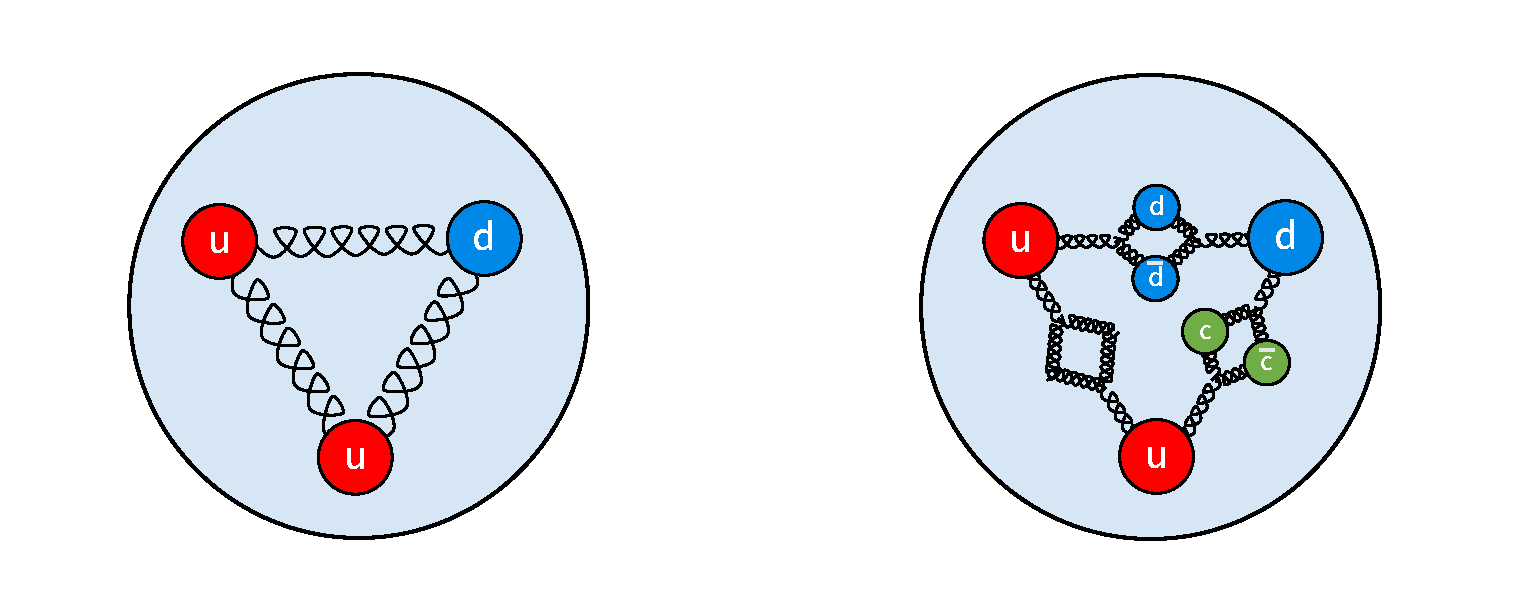
\includegraphics[width=0.75\textwidth]{figures/proton.pdf} 
	}
	\caption{A simple picture of the proton, with three quarks connected by three gluons (left). At shorter timescales, quantum fluctuations exist and the proton picture becomes more complex (right).  }
	\label{fig:proton}
\end{figure}

The linearity of the \ftwo\ structure function was proposed based on the assumption that protons constituents are non-interacting. This ignores QCD radiative processes, the process in which quarks interact with and radiate gluons. Probing the proton at low energies, the picture is one of three partons - two up quarks and a down quark as shown on the left of Fig.~\ref{fig:proton}. These so called valence quarks are strongly interacting and are held together by gluons. However, at smaller distances and shorter timescales, the picture of the proton becomes more complicated, as seen on the right of Fig.~\ref{fig:proton}. In this regime, gluons can be seen splitting into short lived quark-antiquark pairs (sea quarks), or into gluon-gluon pairs. Additionally, it was found that the total momentum contribution of all quarks inside the proton, when the quark PDFs are integrated over a wide range of x, was roughly 50\%~\cite{qcdbook}. All this information strongly suggested the possibility that gluons carry a significant momentum fraction of the proton, depending on the \xb\ and \qsquare\ of the interaction. The inclusion of gluons into the nucleus wavefunction is what gave rise to the scaling violation seen in the various experiments at lower-\xb. As a result, the PDFs for quarks and gluons have to be expressed as a function of \xb\ and \qsquare: $q_{i}(x,Q^{2})$ for quarks and $g_{i}(x,Q^{2})$ for gluons. This new picture of the proton is is sometimes called the $improved\ parton\ model$ or just the parton model, for brevity.

\begin{figure}
	\centering
	\includegraphics[width=0.45\textwidth]{figures/dglap_bfkl.pdf} 
	\caption{ Schematic showing the BFLK evolution in $ln(1/\xb)$ and DGLAP evolution in $ln(\qsquare)$ (left figure). The saturation scale $Q_{S}$ is represented by the diagonal line.}	
	\label{fig:cgc}
\end{figure}

In the regime where pQCD can be used ($\alphaS > \lambda_{QCD}$), techniques have been developed to describe the evolution of PDFs both with \xb\ and \qsquare. The Dokshitzer-Gribov-Lipatov-Altarelli-Parisi (DGLAP) equations~\cite{Gribov:1972rt,Gribov:1972ri,Dokshitzer:1977sg,Altarelli:1977zs} describe the evolution of PDFs at as a function of $ln(\qsquare)$, at a fixed \xb. The other set of equations, describing the PDF dependence on $ln(1/\xb)$ at fixed \qsquare, are the Balitsky-Fadin-Kuraev-Lipatov (BFKL) evolution equations~\cite{Balitsky:1978ic, Kuraev:1977fs, Fadin:1975cb, Lipatov:1976zz}. These sets of equations describing the evolution of parton densities in \qsquare\ and $x$ are considered to be the most fundamental equations in pQCD. The BFLK equation will be of particular interest to this thesis because of its role in evolving PDFs to low-\xb. A schematic representation of the BFLK and DGLAP evolutions in the $ln(1/x)$ vs $ln(\qsquare)$ phase-space is shown in~\ref{fig:cgc}.

\begin{figure}
	\centering
	\includegraphics[width=0.48\textwidth]{figures/d15-039f54a.pdf} 
	\includegraphics[width=0.48\textwidth]{figures/d15-039f55a.pdf} 
	\caption{PDFs obtained at different $Q^{2}$ by the H1 and ZEUS collaborations. The gluon PDFs are scaled so they would fit on the plots with the quark PDFs. Note that the observable plotted is $xq_{i}(x,\qsquare)$. Figure taken from Ref.~\cite{Abramowicz:2015mha}.}	
	\label{fig:pdfsintro}
\end{figure}

Over time, global QCD analysis of structure functions in deep inelastic lepton-nucleon scattering at HERA, as well as jet and hadron cross sections at the LHC, Tevatron, and RHIC were performed in a wide kinematic range, providing several new sets of PDFs with the highest degree of precision reached so far~\cite{Dulat:2015mca,Ball:2017nwa,Harland-Lang:2014zoa,Abramowicz:2015mha}. Examples of quark and gluon PDFs from DIS experiments at different $Q^{2}$ from the H1 and ZEUS collaborations are shown in Fig.~\ref{fig:pdfsintro}. These global QCD analyses show that the \gx\ found to rise rapidly at small \xb\ in the proton. The rapidly increasing \gx\ at $\xb \ll 1$ is explained by gluon radiation (bremsstrahlung) of soft gluons, where a parton with high-\xb\ collinearly emits a gluon with an $\xb_{1} \ll 1$ and with small \pt. This process is shown in Fig.~\ref{fig:bfkllowx} where a soft gluon radiates a softer gluon and this continues with a probability $\propto ln(1/\xb)$ at each step via the BFLK evolution. Naturally, the momentum fraction \xb\ carried by some intermediate gluon in this cascade is smaller than that of its predecessors ($\xb \ll \xb_{n} \ll \xb_{n-1} \ll ... \ll \xb_{2} \ll \xb_{1}$). This divergent behavior of \gx\ means that at small enough \xb, the number of gluons $x\gx$ will tend to infinity. However, unitarity requires that the first moment of the gluon momentum distribution remains finite. Therefore, the steep rise at low-\xb\ must change at some \xb\ value; this possible phenomenon is known as \textit{saturation}~\cite{Gribov:1984tu}. Presently it is believed that the mechanism for saturation is gluon recombination ($g + g\rightarrow g$), which is expected to happen at the  saturation scale $Q_{s}(\xb)$ when the gluon wavefunctions begin to overlap due to very high gluon densities~\cite{Mueller:1985wy}. Gluons with $\pt < Q_{S}$ are said to be at saturation since  their densities do not grow anymore. The phenomenon of saturation, which is the main focus of this thesis, will be discussed in more detail later in this chapter. First, it is informative to learn about some of the tools that can possibly be used to probe this effect. 

\begin{figure}
	\centering
	\includegraphics[width=0.7\textwidth]{figures/bfkl.pdf} 
	\caption{ Graphic representation of BFKL evolution leading to high gluon densities at low-\xb. Figure taken from Ref.~\cite{Iancu:2012xa}.}	
	\label{fig:bfkllowx}
\end{figure}

% In order to better understand how to go about the search for saturation, it is useful to first discuss the tools which will be used to "see" quarks and gluons.

\FloatBarrier

\section{ Hadronic Collisions and Jets }

The DIS experiments successfully showed the scaling violation of the linearity of \ftwo\ with \qsquare\ with smaller-\xb\ and provided precise PDFs for quarks. Indirect measurements of the gluon distribution from \ftwo\ data were still carried out, but the precision on \gx\ was limited because the photon cannot couple with gluons. Fortunately, collisions involving hadrons with hadrons, or hadrons with heavy ions open up the possibility of a hard scattering via gluon, analogous to the interaction via photon in DIS. Since gluons can couple to other gluons, hadronic collisions can be used as direct probes of \gx, providing measurements of the gluon distribution with much higher precision than in DIS. In a collision between two protons, modelled $P_{A} + P_{B} \rightarrow q_{1} + q_{2}$ and shown in the left of Fig.~\ref{fig:hadroniccollisions}, the cross section for a hard scattering process can be written~\cite{qcdbook}

\begin{equation}
\sigma(P_{1}, P_{2}) = \sum_{i,j}^{}\int_{}^{}dx_{1}dx_{2}f_{i}(x_{1},\mu^{2})f_{j}(x_{2},\mu^{2})\sigma_{ij}(p_{1},p_{2},\alphaS(\mu^2), \qsquare/\mu^{2}),
\end{equation}

where $P_{1}$ and $P_{2}$ are the four-momenta of the incoming protons, $p_{1}=x_{1}P_{1}$ and $p_{2}=x_{2}P_{2}$ are the four momenta of the partons participating in the interaction. The quark and gluon PDFs are $f_{i}$ and $f_{j}$, the QCD scattering cross section for partons of type $i$ and $j$ is $\sigma_{ij}$. The hard scattering scale \qsquare\ is determined experimentally and places a lower limit on the possible final state particles that are produced. As discussed previously, at sufficiently high \qsquare, \alphaS\ becomes small, and the cross section can be calculated perturbatively in a series of \alphaS. The factorization scale $\mu^{2}$ is an arbitrary parameter that places an energy threshold on what physics is considered part of the hadron wavefunction and what physics is part of the scattering process and can be considered in the hard scattering cross-section. The dependence on $\mu^{2}$ gets smaller by including more terms in the perturbative expansion of the cross section calculation (which requires more computing power). In general, the factorization scale should be chosen to be $\mu^{2} \sim \qsquare$. 

\begin{figure}
	\centering
	\includegraphics[width=0.7\textwidth]{figures/hadronic_collision.pdf} 
	\caption{ Diagram of a hadronic collision ($P_{A} + P_{B} \rightarrow q_{1} + q_{2}$) between two protons, producing two outgoing partons, which are represented in their final state as a stream of particles. The box represents the hard scattering process.}
	\label{fig:hadroniccollisions}
\end{figure}

A particle collision with sufficiently high energy transfer can result in a quark or gluon being ejected from the hadron in which it was confined. From the properties of confinement, a parton cannot exist alone at macroscopic distances, meaning a quark or gluon cannot be directly observed in a detector. The DGLAP formalism describes the evolution of the ejected parton from the hard scale until the perturbative limit $\lambda_{QCD}$. From QCD rules, as the distance of the exiting parton from its scattering event begins to increase, the probability for radiating collinear gluons will increase. These radiated gluons can in turn split into quark antiquark pairs, which can radiate more gluons, and so fourth. The quarks and antiquarks from the resulting cascade then recombine into color singlet states of particles  collienar with the original parton.  This process, known as $hadronization$, produces a narrow cone of particles called $jets$~\cite{Sterman:1977wj, Webber:1983if, Andersson:1983ia}. The creation of these final state particles that make up a jet is described by phenomenological models, since at every level in the hadronization process, the energy of the newly created partons decreases until perturbative methods can no longer be applied. Many of these newly created particles have a lifetime sufficiently long enough for them to reach and create a signal in a detector. In this sense, a jet is a manifestation of a parton that was knocked out in a scattering event, however the precise definition of a jet depends on the procedure with which it is reconstructed. An example of an actual event from ATLAS where two jets (dijets) were created and reconstructed is shown in Fig.~\ref{fig:atlasjets}.

\begin{figure}
	\centering
	\includegraphics[width=0.7\textwidth]{figures/jets.pdf} 
	\caption{ Event display from a real ATLAS dijet event. Shown are two back-to-back jets, which are manifestations of the quarks involved in a hard scattering at the interaction point, which is labeled in the figure. }
	\label{fig:atlasjets}
\end{figure}


\subsection{\mbox{Anti-\kt} Jets} 
Before a jet's energy and position can be correctly described, a prescription of what a jet is must be agreed upon. A jet can have many constituents, which are final state particles produced in the hadronization process. These particles can be physically detected and used as input into clustering algorithms that aim to describe jets consistent with theory predictions~\cite{Ellis:1993tq,Dokshitzer:1997in,Wobisch:1998wt,Blazey:2000qt}. While different algorithms have their advantages and disadvantages, the \antikt\ algorithm~\cite{Cacciari:2008qp} has grown in popularity since its introduction almost a decade ago. Besides its fast computation speed, the main advantage of the \antikt\ algorithm is its infrared and collinear safety (IRC) from effects of soft radiation.

Any jet clustering algorithm needs to accept a set of homogeneous input data (objects) such as the four-momenta of particles, calorimeter tower energies, topological calorimeter cells, etc. The treatment of these input objects by the algorithm is identical. The \antikt\ algorithm comes from a broader family of \kt\ clustering algorithms that appear the same in their formalism but yield different results based on an important parameter that will be discussed shortly. The general form of any \kt\ algorithm involves a collection of input objects with indexes $i$ having energy and spatial coordinates $(\eta_{i}, \phi_{i}, p_{\mathrm{T}_{i}})$ where $\eta_{i}$, $\phi_{i}$, and $\pt_{i}$ are the objects pseudorapitidy, azimuthal angle, and transverse momentum, respectively. Between any two objects $i$ and $j$, two distances are defined in terms of energy and position:

\begin{equation}
	d_{iB} = -p^{2p}_{\mathrm{T}_{i}}
	\label{diB}
\end{equation} 
\begin{equation}
	d_{ij} = min( p^{2p}_{\mathrm{T}_{i}}, p^{2p}_{\mathrm{T}_{j}})\frac{\Delta R}{R^{2}}
	\label{dij}
\end{equation}

where $\Delta R^{2} = (\eta_{i} - \eta_{j} )^2 - ( \phi_{i} - \phi_{j} )^2$, $R$ is the characteristic radius parameter describing the maximum allowed radius of a jet, and the parameter $p$ is what determines which type of \kt\ algorithm is used. The general prescription for any \kt\ algorithm is as follows:

\begin{enumerate}
	\item Out of the list of objects, calculate all distances $d_{ij}$ and $d_{iB}$.
	\item Identify the smallest distance out of $d_{ij}$ and $d_{iB}$.
	\item If the minimum is $d_{ij}$, combine the four-momenta of the $i^{th}$ and $j^{th}$ objects, return to the first step, and begin again.
	\item If the minimum is $d_{iB}$, save object $i$ as a jet and remove it from the list of objects. Then return to the first step and begin again.
	\item Continue this process until the list of objects is empty.
\end{enumerate}

The behavior of all the \kt\ algorithms with respect to soft radiation is the same for any $p < 0$ but the focus is going to be on the case of $p = -1$, which is the parameter used in the \antikt\ jet reconstruction algorithm mentioned earlier. To understand the general idea of how it works, it is useful to begin with an ensemble several high \pt\ (hard) objects, and many low \pt\ (soft) objects used as an input to the algorithm. The distance $d_{ij}$ between a hard particle $i$ and a soft particle $j$ will dominated by the hard particle $i$ and will be smaller than the distance $d_{kl}$ between two soft particles $k$ and $l$. This means that soft objects will cluster with hard objects preferentially over other soft objects. If the hard object $i$ has no other hard object within a distance of $2R$, all soft objects within a circle of radius $R$ will simply cluster with object $i$ and eventually form a perfectly conical jet of radius $R$. If there are two had particles with $\Delta R < R$, then they will be combined to form a jet of radius $R$ around the higher \pt\ object. If object $i$ has another hard object within $R < \Delta R < 2R$, the object with higher \pt\ will form a perfectly conical jet of radius R, and the object with lower \pt\ will form a jet an area clipped by its neighbor with higher \pt. In reality, it does not matter what object is hard or soft, the algorithm takes a list of objects as input, naturally performs the clustering of these objects according to its prescription, and outputs a collection of jets. An example of the same input data run through different jet reconstruction algorithms is shown in Fig~\ref{fig:jetalgos}. The \antikt\ algorithm was adopted by ATLAS as a standard way to describe jets due to its IRC safety, fast performance, and robust treatment of various kinds of input datasets. 

\begin{figure}
	\centering
	\includegraphics[width=0.75\textwidth]{figures/jetalgo.pdf} 
	\caption{ Results of jet reconstruction by the \kt\ (top left), Cambridge Aachen (top right), SISCone (bottom left), and \antikt\ (bottom right) algorithms on identical input sets with a jet radius requirement of \ROne. Figure taken from Ref.~\cite{Cacciari:2008qp}.}
	\label{fig:jetalgos}
\end{figure}

\FloatBarrier

\section{Gluon Saturation}
The search for the onset of saturation was first pursued with $d+\mathrm{Au}$ collisions at RHIC~\cite{Adler:2003au, Wang:2007zv, Adare:2011sc}, where the sensitivity to possible saturation effects was increased due to the enhancement of the nuclear gluon density in the Lorentz-contracted heavy ion nucleus~\cite{Albacete:2014fwa,Blaizot:2016qgz}. More recent measurements at the LHC have been performed in the proton-going direction of \pPb\ collisions and at higher center-of-mass energies, allowing lower-\xb\ of the lead nucleus to be probed~\cite{ATLAS:2014cpa, Adam:2015xea, Adam:2015hoa, Khachatryan:2016xdg}. The ALICE measurement of dijet azimuthal correlations at mid-rapidity did not find significant modification in \pPb\ collisions compared to \pp\ collisions. The ATLAS and CMS measurements of inclusive jet production also did not find significant evidence of nuclear modification. Recently, CMS extended the search for gluon saturation to the highest gluon densities reached so far by measuring the inclusive jet cross-section in \pPb\ collisions at very forward rapidity using the CASTOR detector with $-6.6 < \eta < -5.2$, probing $x$ down to $10^{-6}$~\cite{VanDeKlundert:2017ulj}. Comparing measured jet \pt\ spectra to event generators (\textsc{Epos-lhc}~\cite{PhysRevC.92.034906}, \textsc{Hijing}~\cite{PhysRevD.44.3501}, and \textsc{Qgsjetii-04}~\cite{qgsjet}), it was found that none could describe the data over the full jet \pt\ spectra range, opening up the possibility for nuclear effects not described by these models. Currently, the differences between nuclear PDFs (nPDFs) and free nucleon PDFs are often understood from shadowing, anti-shadowing, and EMC effects~\cite{Eskola:2016oht,Kovarik:2015cma}. Calculating nPDFs  $f_{i}^{A}( \xb, \qsquare )$ for parton types $i$ from $F_{2}^{A}$ of heavy ions with atomic number $A$ and comparing them to free nucleon PDFs $f_{i}^{p}( \xb, \qsquare )$ calculated from $F_{2}^{p}$ is direct measure of the nuclear modification factor

\begin{equation}
	R^{A}_{i} = \frac{f_{i}^{A}( \xb, \qsquare )}{A f_{i}^{p}( \xb, \qsquare )}.
\end{equation}

Studies of nPDFs in heavy ion nuclei expected a scaling of free nucleon PDFs with $A$ such that the nuclear modification factor is consistent with unity. The parameterization of $R_{i}^{A}$ shown in Fig~\ref{fig:shadowing} indicates that the nuclear modification factor is not consistent with unity at various values of \xb. The suppression of $R^{A}_{i}$ can be seen from shadowing (low-\xb) and EMC($\xb~\sim 1$) effects, while enhancement of $R^{A}_{i}$ can be seen from the antishadowing effect at $\xb~\sim 10^{-1}$. The shadowing effect, which is of most interest to the low-\xb\ physics of this thesis, is thought to arise from screening of the nuclear parton densities by gluons on the outside of the heavy ion nucleus, which interact preferentially with any incoming probes. While this effect is not completely understood, it is well known experimentally. As discussed earlier, the large uncertainty on the gluon nPDFs and free nucleon gluon PDFs is due to the inability to directly probe gluon densities from \ftwo. Additionally, final state processes can also contribute to the modification of the gluon nPDF. This opens up the possibility for additional nuclear processes to contribute to the gluon density suppression at low-\xb.

\begin{figure}
	\centering
	\includegraphics[width=0.7\textwidth]{figures/shadowing.pdf} 
	\caption{ Illustration of a generalized EPPS16 parameterization of the nuclear modification factor $R^{A}_{i}$ for different parton types $i$ and heavy ions with atomic number $A$. Suppression of $R^{A}_{i}$ by nuclear shadowing and EMC effects are prevalent at low- and high-\xb. Enhancement of $R^{A}_{i}$ due to antishadowing effects are seen in an intermediate-$x$ range. Figure taken from Ref.~\cite{Eskola:2016oht}. }	
	\label{fig:shadowing}
\end{figure}

\FloatBarrier
\section{Color Glass Condensate}

One of the proposed models of gluon saturation is in the framework of the Color Glass Condensate (CGC)~\cite{Iancu:2002xk, Kharzeev:2004bw, Gelis:2012ri}. It is useful to discuss the meaning of the name: $color$ comes from the fact that gluons carry a color charge, $glass$ describes how short lived gluons with low-\xb\ see the surrounding higher-\xb\ gluons in the dense medium as "frozen", $condensate$ describes the saturated nature of the high density gluons recombining with one another. The CGC effective theory describes a model for the interaction of a high energy parton with a highly dense gluon medium described by the BFKL evolution that includes a non-linear term responsible for gluon recombination. In the schematic shown in Fig.~\ref{fig:cgcfield}, a low-\xb\ gluon that originated or re-scattered from other gluons with higher $x' > \xb$ is emitted and interacting with this gluon is a probe of the overall gluon field $A(\rho)$, where $\rho$ is the color charge density of the nucleon. Recently, together with non-relativistic QCD, the CGC model was able to successfully describe experimental data on the cross section of $J/\psi$ production at ALICE~\cite{Weber:2017kjj}, shown in Fig.~\ref{fig:jpsialice}.

%single model for a many body self-interacting system of highly dense gluons

\begin{figure}
	\centering
	\includegraphics[width=0.65\textwidth]{figures/cgc_field_2.pdf} 
	\caption{ Schematic representation of the CGC theory, showing the high density, low-\xb\ gluons originating from high-\xb\ partons (left). These gluons form a gluon field $A{\rho}$ where the whole gluons with higher-\xb\ are represented by a color charge density $\rho$. Figure taken from Ref.~\cite{Iancu:2012xa}. }	
	\label{fig:cgcfield}
\end{figure}


\begin{figure}
	\centering
	\includegraphics[width=0.65\textwidth]{figures/jpsialice.pdf} 
	\caption{ Figure taken from Ref.~\cite{Weber:2017kjj}. }	
	\label{fig:jpsialice}
\end{figure}

A measurement probing gluon saturation in nuclear gluon densities in the framework of the CGC model was  was proposed by measuring possible modifications of dijet azimuthal angular distributions in \pPb\ and \pp\ collisions at an $x$ down to $10^{-5}$~\cite{vanHameren:2014lna,}. For back-to-back dijets, the gluon field in the Pb nucleus is probed at low transverse momentum where saturation effects are expected to be large. These effects are described by whether or not an incoming parton scatters individually off each gluon in the highly dense field of the lead nucleus, or recoils against the nucleus as a whole. An away-side jet is created when a constituent gluon of this dense field is knocked out of the nucleus by the scattering incoming parton. However, due to the highly dense field, the incoming parton can scatter many times, losing energy and changing trajectory. As a result, if there are two outgoing jets, one from the scattered parton, and the other jet (away side) from a knocked out gluon, they may not be perfectly back-to-back, resulting in the azimuthal broadening. The monojet signature could result from the incoming parton recoiling off the nucleus coherently~\cite{Kharzeev:2004bw}. The parton would not scatter with any of the individual partons, and as a result, would not produce an away-side jet. To probe these effects, one must define some observables, which will be extracted from data and presented in the latter sections of this thesis.

\section{Measured Observables}

This thesis will present a  measurement of dijet production at forward rapidity with the ATLAS detector. Proton-lead collisions are studied in addition to proton-proton collisions because of the enhancement of gluon densities in the Lorentz contracted lead nucleus.


At the leading order, in a hard scattering event between a proton moving in the $+z$ direction, and a lead nucleus moving in the $-z$ direction, as shown in the middle panel of Fig.~\ref{fig:yandystar}, there will be two outgoing partons, one with transverse momentum \ptone\ and center-of-mass rapidity \ystarone\ coming from the proton, and one with transverse momentum \pttwo\ and center-of-mass rapidity \ystartwo\ coming from a nucleon in the lead ion. The center-of-mass rapidities ($\ystar \equiv y - \Delta y$) are used to account for the rapidity shift of the center-of-mass frame of the \pPb\ system relative to the ATLAS laboratory frame. The resulting expressions for parton momentum fractions $x_{p}$ of the proton's parton, and $x_{\mathrm{Pb}}$ of a lead nucleon's parton will be:

\begin{equation}
x_{p}=\frac{\ptone e^{\ystarone}+\pttwo e^{\ystartwo}}{\sqrt{s}}, \ \ x_{\mathrm{Pb}}=\frac{\ptone e^{-\ystarone}+\pttwo e^{-\ystartwo}}{\sqrt{s}}.
\label{eqn:x1x2}
\end{equation}

From these equations, it is clear that to probe a lower $x_{\mathrm{Pb}}$, two forward (high \ystarone and \ystartwo) particles, with low \ptone\ and \pttwo\ are preferred. To show the difference between rapidity $y$ and center-of-mass rapidity \ystar, an event producing two jets in \pp\ collisions is shown on the left panel of Fig.~\ref{fig:yandystar}. The azimuthal angle \Dphi\ between two jets is shown on the right panel of  Fig.~\ref{fig:yandystar}

\begin{figure}
	\centering
	\includegraphics[width=0.970\textwidth]{figures/collision_system.pdf} 
	\caption{Example of a collision in the $y-z$ plane in \pp\ where $y=\ystar$ (left), a collision in the $y-z$ plane in \pPb\ where $\ystar \equiv y - \Delta y$ (middle) to account for the boost ($\Delta y$) of the center-of-mass system, and a collision in the $x-y$ plane showing the difference in azimuthal angle \Dphi\ between two jets (right). }	
	\label{fig:yandystar}
\end{figure}

\begin{figure}
	\centering
	\includegraphics[width=0.40\textwidth]{figures/kutak0.png} 
	\includegraphics[width=0.40\textwidth]{figures/kutak1.png} 
	\caption{ Dijet azimuthal angular correlations from theoretical models for central-forward \pp\ and \pPb\ collisions as a function of \Dphi\ between two jets in different \pt\ bins. Figure taken from Ref. ~\cite{Kutak:2012rf}. }	
	\label{fig:kutakdphi}
\end{figure}

The final observables in this analysis are dijet azimuthal angular \Dphi\ distribution widths and conditional yields of dijets.  Example dijet \Dphi\ distributions are shown from theoretical models in Figure~\ref{fig:kutakdphi}. The measurement is performed in different intervals of \ystarone, \ystartwo, \ptone, and \pttwo, where \ystarone, \ptone\ is the center-of-mass rapidity and transverse momentum of the leading jet, and \ystartwo, \pttwo\ the  center-of-mass rapidity and transverse momentum of the sub-leading jet. The leading jet, which is required to be in the forward (defined as proton-going) direction, has the highest \pT\ in the event, and the sub-leading jet has the second highest \pT\ in the event. This is a measurement of dijets probing the lowest-\xb\ of the lead nucleus at the hardest scattering scale so far. The azimuthal angular correlation functions, \conetwo, which are normalized to the number of leading jets, are defined as

\begin{equation}
\conetwo=\frac{1}{N_{1}} \frac{\mathrm{d}N_{12}}{\mathrm{d}\Dphi},
\label{eqn:c12}
\end{equation}

where $N_{1}$ is the number of leading jets, $N_{12}$ is the number of dijets, and \Dphi\ is the lower azimuthal angle between the leading and sub-leading jets. The \conetwo\ distributions are fitted and their widths \wonetwo\ defined by the root-mean-square (RMS) of the fit: \wonetwo = RMS(\conetwo).

In addition to dijet azimuthal angular distributions, the dijet conditional yields, \ionetwo, are measured and defined as

\begin{equation}
\ionetwo=\frac{1}{N_{1}}  \frac{\mathrm{d}N_{12}}{\mathrm{d}\ystarone\mathrm{d}\ystartwo\mathrm{d}\ptone\mathrm{d}\pttwo}.
\label{eqn:ippb}
\end{equation}

where \ptone, \pttwo, \ystarone, and \ystartwo\ are the transverse momenta and center-of-mass rapidities of the leading and sub-leading jets, respectively. 

The azimuthal angular correlations and conditional yields evaluated in \pPb\ and \pp\ collisions are compared and the ratios in \wonetwo\ and \ionetwo\ between the two systems are calculated as:

\begin{equation}
\cppb=\frac{W_{12}^{\pPb}}{W_{12}^{\pp}} \ \ , \ \ \ippb=\frac{I_{12}^{\pPb}}{I_{12}^{\pp}}.
\end{equation}

Finding a broadening in the dijet angular correlation distribution for \pPb\ collisions compared to \pp\ collisions probes for nuclear effects in the jet formation and scattering off individual gluons of the highly dense gluon field. A suppression of the conditional yields in \pPb\ compared to \pp\ could be an indicator of the mono-jet or jet quenching event signature due to the coherent scattering off the lead nucleus as a whole.

To closer follow next-to-leading-order (NLO) calculations, a minimum $\Delta \pT=\ptone - \pttwo$ is required on the dijets~\cite{Potter:1999gg,Klasen:1995xe,Frixione:1997ks}. However, techniques such as Sudakov re-summation~\cite{Bury:2017jxo} can take into account the absence of $\Delta \pT$ requirements. Also, comparisons with fixed-order calculations and soft gluon re-summation, which involve transverse momentum dependent PDFs, instead of collinear PDFs, are better suited for scenarios not requiring any minimum $\Delta \pT$ cut. The results of the measurement are therefore presented both without any requirement on $\Delta\pT$, as well as with the requirement of $\Delta\pT>3$ GeV.

\FloatBarrier
